\documentclass[conference]{IEEEtran}
\IEEEoverridecommandlockouts
%% ---------------------------------------------------------------------------
%% Glaukopis: Building a 32B CTI LLM Using Multi-Stage Instruction Fine-Tuning
%% IEEE Conference template port — targets 38th IEEE ICTAI 2026
%% (https://ictai.computer.org/2026/)
%%
%% Worth, Cardei, Alam. Compile with pdfLaTeX:
%%   pdflatex glaukopis_ieee
%%   bibtex   glaukopis_ieee
%%   pdflatex glaukopis_ieee
%%   pdflatex glaukopis_ieee
%% ---------------------------------------------------------------------------

\usepackage{cite}
\usepackage{amsmath,amssymb,amsfonts}
\usepackage{algorithmic}
\usepackage{graphicx}
\usepackage{textcomp}
\usepackage{xcolor}
\usepackage{url}
\usepackage{hyperref}
\usepackage{booktabs}
\usepackage{array}

\graphicspath{{figures/}{img/}{Fig/}}

%% --- Technical-identifier macro --------------------------------------------
%% \hfid{...} renders a Hugging Face / Hugging Face-style identifier (model
%% name, dataset path, etc.) in a slightly smaller monospaced font that wraps
%% cleanly at `/`, `-`, and `_` boundaries so that long identifiers do not
%% overflow the column. Implemented via the url package with hyphen and
%% underscore added to the break set.
%% --------------------------------------------------------------------------
\makeatletter
\AtBeginDocument{%
  \urlstyle{tt}%
  \def\UrlBreaks{\do\/\do\-\do\_\do\.\do\:}%
}
\makeatother
\providecommand{\hfid}[1]{{\small\nolinkurl{#1}}}

\def\BibTeX{{\rm B\kern-.05em{\sc i\kern-.025em b}\kern-.08em
    T\kern-.1667em\lower.7ex\hbox{E}\kern-.125emX}}

\begin{document}

\title{Constructing a 32B CTI LLM with a Multi-Stage Instruction Fine-Tuning Framework (Glaukopis)
\thanks{This research was funded by Athena Security Group, LLC.}
}

\author{%
\IEEEauthorblockN{%
  Peter J. Worth Jr.\textsuperscript{1,3,*},\quad
  Ionut Cardei\textsuperscript{1,3},\quad
  Salman Ahmad\textsuperscript{4},\quad
  Muhammad Mamoon Khan\textsuperscript{4}%
}
\IEEEauthorblockA{%
  \textsuperscript{1}\textit{Dept.\ of Electrical Engineering and Computer Science, Florida Atlantic University}, Boca Raton, FL, USA \\
  \textsuperscript{3}\textit{Athena Security Group, LLC}, USA \quad
  \textsuperscript{4}\textit{RevolveAI} \\[2pt]
  \textsuperscript{*}Corresponding author: \texttt{pworthjr@athenasecuritygrp.com}%
}%
}

\maketitle

\begin{abstract}
Cyber threat intelligence (CTI) workflows in regulated security operations may be unable to rely on frontier proprietary models because of cost, latency, or data-handling constraints, while general-purpose foundation models often lack the schema fidelity, applied reasoning, and current-threat awareness needed for operational CTI tasks. This paper presents \textbf{Glaukopis}, a disciplined CTI-specific, multi-stage instruction fine-tuning (IFT) framework for producing on-premises 32-billion-parameter (32B) CTI expert language models. On the data side, declarative graph-query templates are executed against an authoritative knowledge graph and the returned nodes, relationships, and properties are rendered into instruction records; on the training side, the supervised pass is decomposed into stages with purpose-specific data subsets and hyperparameter regimes. Glaukopis has three components: \textbf{Ariadne}, a Neo4j substrate ingesting twelve public CTI sources into ${\sim}280$K nodes and ${\sim}480$K edges; \textbf{Sophia}, a graph-template generator that executes typed queries and renders their results as graph-grounded instruction records; and a \textbf{four-stage IFT schedule} (Core, +TAA, CSE, Recalibrate-32B). The v21 ship checkpoint reaches a 66.3 average CTI benchmark score (vs.\ 59.0 for its Qwen-2.5-32B-Instruct base), approaching DeepSeek-V4-Pro (70.4), Gemini-3-Flash-Preview (69.8), and GPT-5.5 (72.9) at 45--408$\times$ lower full-suite evaluation cost than those three reference models.
\end{abstract}

\begin{IEEEkeywords}
instruction fine-tuning, multi-stage IFT, supervised fine-tuning, small language models, cyber threat intelligence, CTI knowledge graphs, Neo4j, MITRE ATT\&CK, AthenaBench
\end{IEEEkeywords}

\section{Introduction}

Large language models (LLMs) are now embedded throughout the cyber security workflow: they summarize threat reports, map indicators to MITRE ATT\&CK, triage vulnerabilities, draft detection rules, and answer analyst questions inside security operations centers (SOCs). Surveys of security LLMs consistently identify the same residual failure modes: hallucinations on schema-bearing fields, shallow pattern matching where multi-hop reasoning is required, and a structural inability to operate on threat information more recent than the base model's pretraining cutoff \cite{levi2024cyberpal,liu2024cyberbench}.

\textbf{The operational dilemma.} General-purpose models are inexpensive and easy to host, but cyber-specific evaluations show substantially lower performance on schema-bearing and reasoning-intensive tasks such as vulnerability-to-CWE mapping, attack-technique extraction, mitigation recommendation, and threat-actor attribution \cite{alam2024ctibench,alam2025athenabench,liu2024cyberbench}. Hosted frontier models close part of this gap, but external API use may be restricted by organizational policy, contractual controls, or data-residency requirements. Even where such use is permitted, cost remains material: in our full-suite measurement, API-served reference models cost 4--408$\times$ as much as the locally served ship checkpoint (Table~\ref{tab:results-cost}). The deployment choice is therefore a capability--governance--cost trade-off rather than a simple preference for the largest available model.

\textbf{Multi-stage CTI instruction fine-tuning.} A natural alternative is an open-weight model at approximately 32B parameters, post-trained on CTI material from authoritative public sources and deployable on-premises. Glaukopis is not proposed as a new learning algorithm; it is a disciplined CTI-specific framework that applies standard IFT \cite{wei2022flan,ouyang2022instructgpt,chung2022flant5} with two engineering choices: (i) on the \emph{data} side, every instruction record is materialized by a typed query against an authoritative knowledge graph rather than authored or LLM-synthesized, so each row is grounded in named graph nodes and relationships traceable to public-source natural keys; and (ii) on the \emph{training} side, the supervised pass is decomposed into stages with distinct shards (purpose-specific training subsets) and hyperparameter regimes, so gains and regressions can be attributed to particular stages. The closest neighbors are IBM's CyberPal.AI and SecKnowledge, which couple expert-curated instruction schemas with chain-of-thought enrichment \cite{levi2024cyberpal,levi2025toward}, and SEvenLLM and CyberBench, which adapt smaller open models through hand-crafted or LLM-synthesized corpora \cite{ji2024sevenllm,liu2024cyberbench}.

\textbf{The Glaukopis system.} Glaukopis is the working instantiation of this multi-stage CTI IFT framework, with three named components: \textbf{Ariadne} (Section~\ref{sec:cti-kg}), a Neo4j substrate ingesting twelve public CTI sources into ${\sim}280$K nodes and ${\sim}480$K edges, refreshed daily; \textbf{Sophia} (Section~\ref{sec:cti-kg}), a graph-template generator that executes declarative CTI reasoning patterns as typed Cypher queries and renders the returned subgraphs into instruction, optional-context, and target fields; and a \textbf{four-stage IFT schedule} (Section~\ref{sec:glaukopis})---Core, +TAA, CSE, Recalibrate-32B---each with its own shard, hyperparameter regime, and intended capability outcome (Figure~\ref{fig:glaukopis-chained-ift}). The canonical 32B schedule permits up to 379,600 examples across five optimization passes (Stage~1 has two phases); Section~\ref{sec:glaukopis} gives the per-pass sample caps and token limits.

\textbf{Headline result.} The released v21 ship checkpoint \cite{glaukopis2026model} reaches an average CTI-benchmark score of 66.3 across AthenaBench, CyberSOCEval, and CyberMetric---7.3 points over its Qwen-2.5-32B-Instruct base (59.0), without changing parameter count or runtime footprint. It exceeds Gemini-2.5-Flash (63.4), runs essentially even with DeepSeek-V3.2-Exp (66.0), and sits within 4--7 points of the leading frontier references---DeepSeek-V4-Pro (70.4), Gemini-3-Flash-Preview (69.8), and GPT-5.5 (72.9)---at 45--408$\times$ lower full-suite evaluation cost than those three models (Section~\ref{sec:results}).

\textbf{Contributions.} (1) We present a CTI-specific multi-stage IFT framework that combines graph-grounded data construction with staged supervised training, and locate it within the FLAN/InstructGPT/FLAN-T5 lineage and the CyberPal.AI/SecKnowledge line. (2) We describe Ariadne and Sophia, a complete, auditable training-data pipeline in which every row maps to specific public-source identifiers. (3) We specify and release a four-stage IFT recipe with per-stage data definitions, sample caps, token limits, and optimization hyperparameters. (4) We report per-stage ablations and cross-architecture transfer across AthenaBench, CyberSOCEval, CyberMetric, and MMLU-Pro, together with a cost analysis and an explicit contamination-control protocol. (5) We release source and checkpoints at \url{https://github.com/Athena-Software-Group/Glaukopis} \cite{glaukopis2026repo}.

\begin{figure*}[t]
\centering
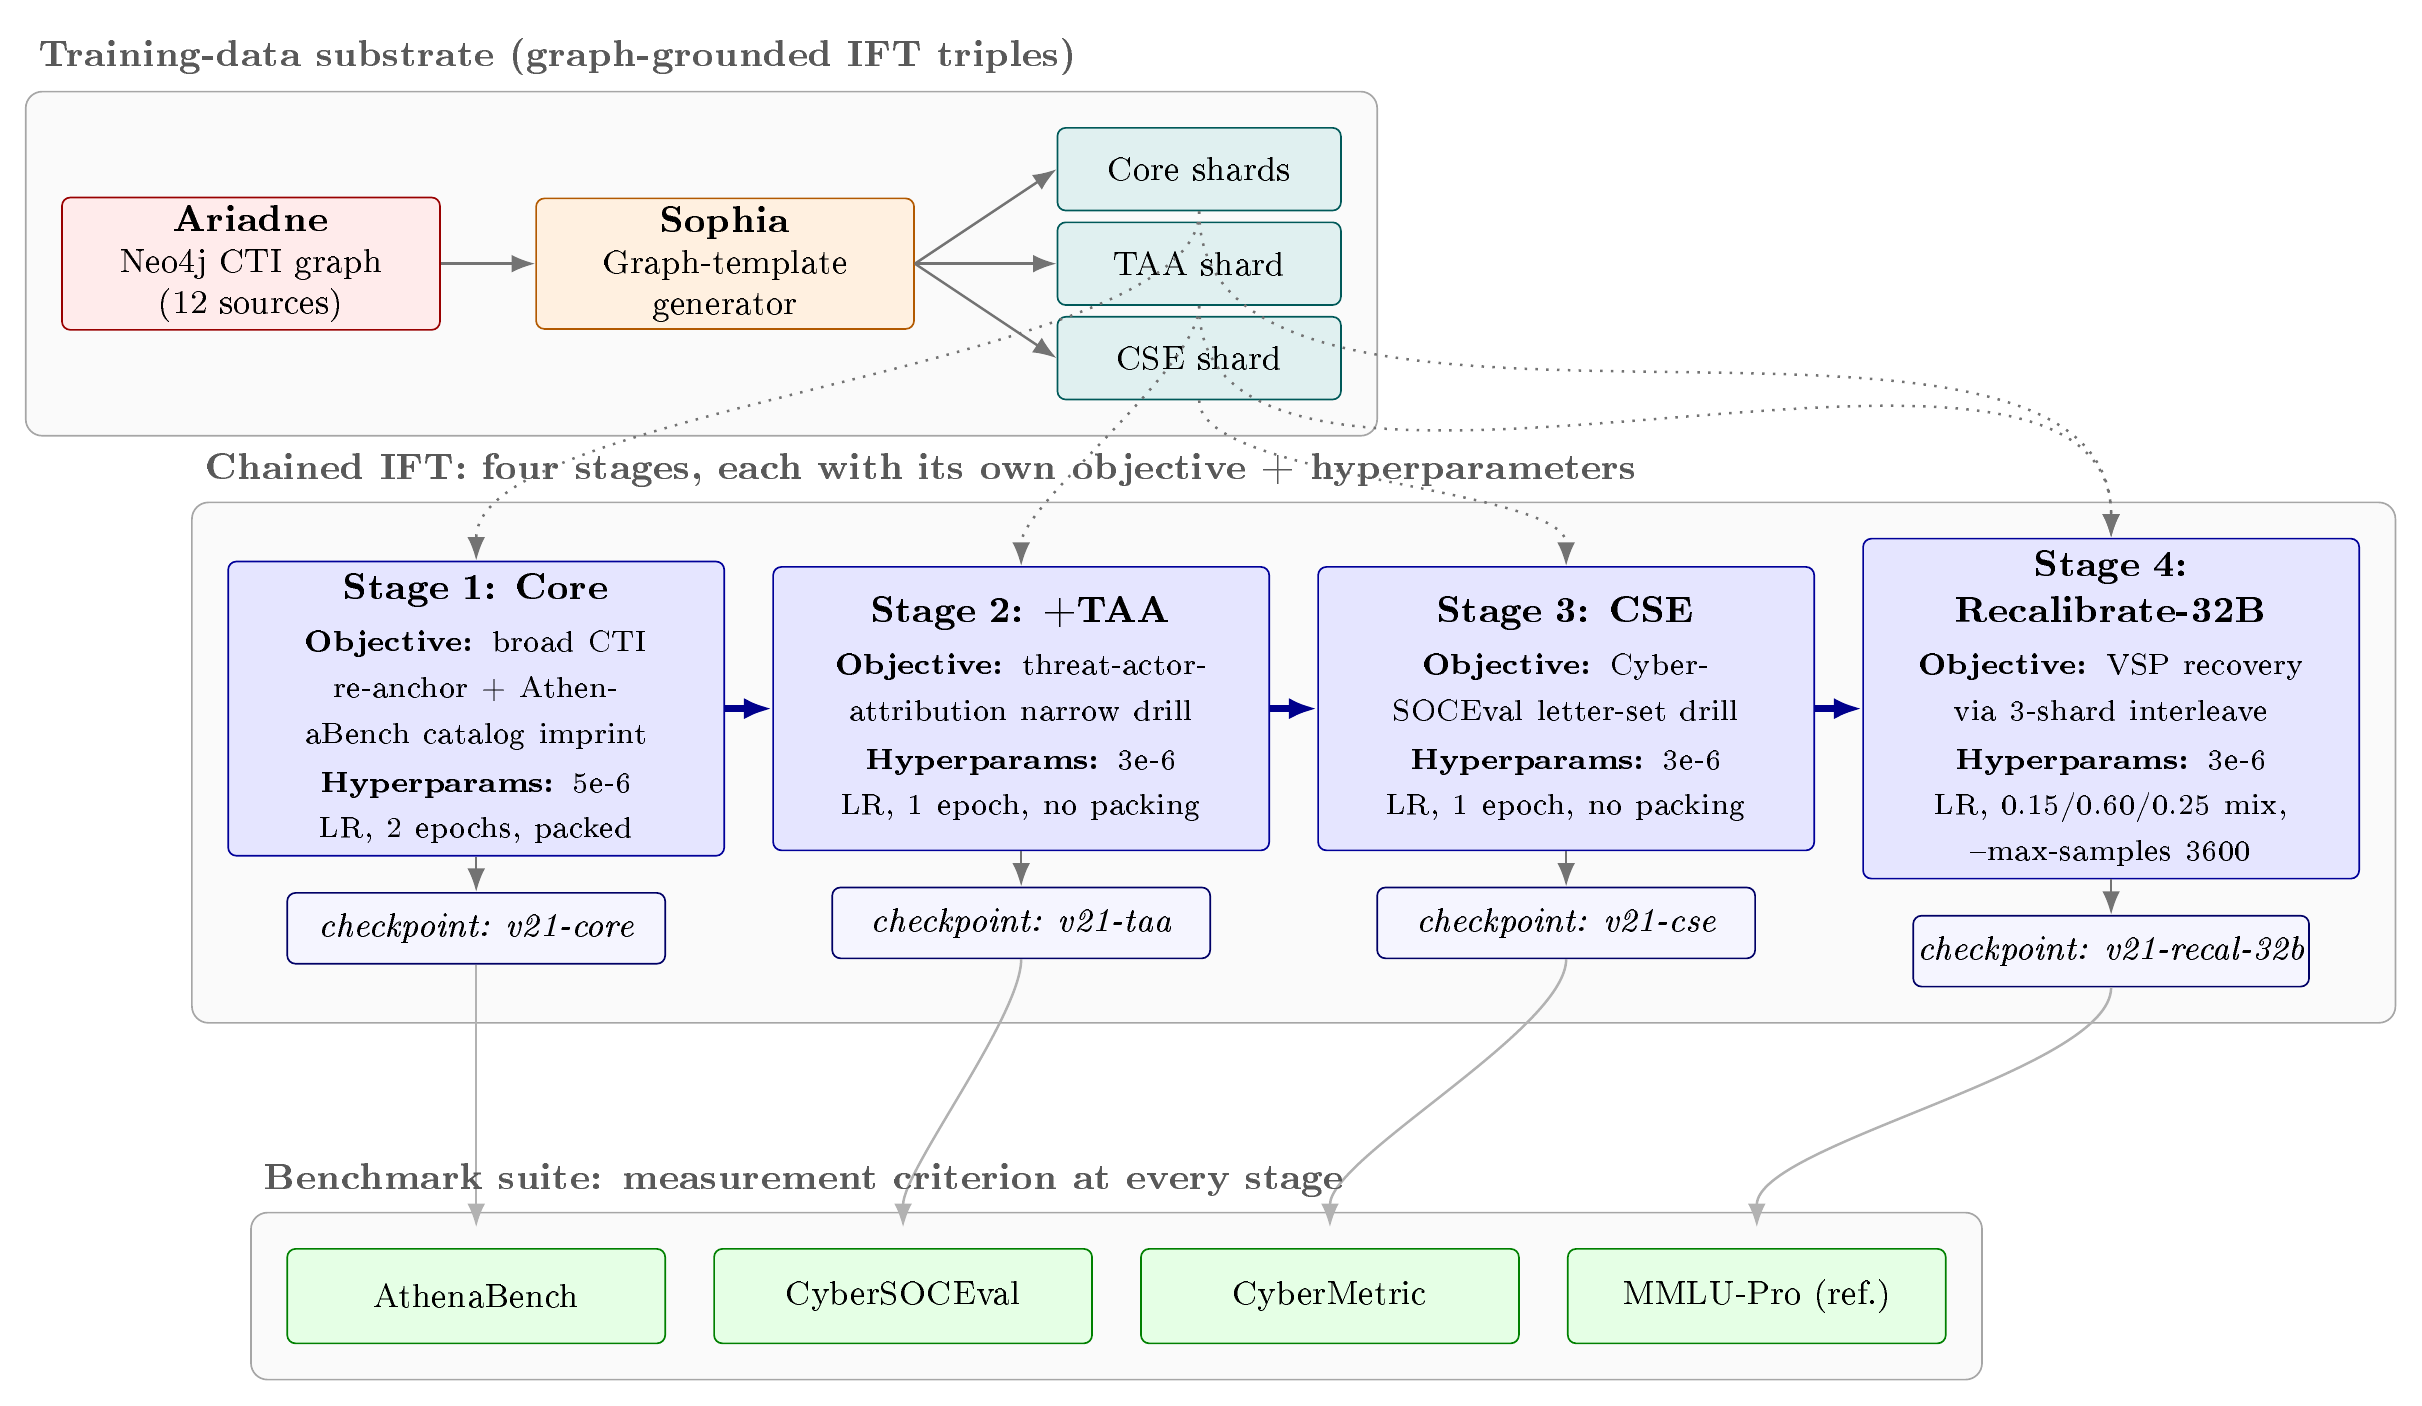
\includegraphics[width=\textwidth]{figures/glaukopis_chained_ift.png}
\caption{\textbf{The multi-stage CTI IFT pattern.} Sophia executes typed graph-query templates against Ariadne and produces graph-grounded instruction records, grouped into Core, TAA, and CSE shards (purpose-specific subsets). The four-stage schedule consumes these in order: each stage has its own objective (broad CTI re-anchoring for Core, narrow drills for TAA and CyberSOCEval, and recalibration for Stage~4) and its own hyperparameters. A cumulative checkpoint is retained after Core, +TAA, CSE, and Recalibrate-32B, and each is evaluated against AthenaBench, CyberSOCEval, CyberMetric, and MMLU-Pro to support per-stage tracking as well as selection of one ship checkpoint.}
\label{fig:glaukopis-chained-ift}
\end{figure*}

\section{Background and Related Work}
\label{sec:ift-slm}

\textbf{IFT foundations.} Instruction fine-tuning (IFT) adapts a pretrained LLM on labeled (instruction, optional context, target) data, maximizing log-likelihood of the reference output \cite{wei2022flan,ouyang2022instructgpt}; it is one instantiation of supervised fine-tuning (SFT), and we use ``IFT'' following the cyber security literature. FLAN \cite{wei2022flan} established that instruction-following is a \emph{learnable} capability rather than a pure emergent of scale. InstructGPT \cite{ouyang2022instructgpt} introduced the staged SFT$\to$preference$\to$RLHF pipeline and showed that small instruction-tuned models can be preferred over much larger unaligned ones---the load-bearing argument for the small-model strategy here. FLAN-T5 \cite{chung2022flant5} scaled the instruction corpus to thousands of tasks and showed that instruction-data diversity and structure matter at least as much as parameter count, licensing the Glaukopis choice to invest in instruction-data structure at a fixed 32B budget.

\textbf{Multi-stage IFT.} A recurring choice in modern post-training is to compose several IFT stages rather than a single monolithic tune: the output of each stage initializes the next, stage effects become easier to observe, and individual stages can be re-run when their data changes. Separating broad domain absorption from precise task behavior can reduce destructive interference \cite{gururangan2020dontstop,ouyang2022instructgpt}; reasoning supervision is more effective layered on top of a model that already commands the domain vocabulary \cite{wei2022cot,levi2025toward}; and staging makes pipelines incrementally refreshable, which matters where source data turns over weekly. Glaukopis adopts a four-stage schedule (Core, +TAA, CSE, Recalibrate-32B); the CyberPal.AI/SecKnowledge line operationalizes a related staging discipline on a different data pipeline \cite{levi2024cyberpal,levi2025toward}.

\textbf{Graph-grounded IFT.} The second refinement is on the data side: every instruction record is materialized by a typed query against an authoritative knowledge graph. This converges three lines: schema- and grammar-constrained generation (targets computed by executing queries against a reference database rather than authored); knowledge-graph-grounded question answering, where a typed traversal returns a subgraph rendered into a question-and-answer (Q\&A) pair (CTI instantiations include \cite{fieblinger2024kg,wu2022opencykg,yu2024ctikg,zhao2024kctiaa,zhang2023cyberkg}); and expert-schema-driven IFT for cyber security \cite{levi2024cyberpal,levi2025toward}. Glaukopis combines all three: the Ariadne schema defines the typed substrate, every Sophia row is materialized by a Cypher query against the populated graph, and the driving templates are expert-authored CTI reasoning patterns.

\textbf{IFT and SLMs for cyber security.} Cyber security imposes heterogeneous schemas (CVE, CWE, CAPEC, ATT\&CK), evidence-grounded structured outputs, and rapid concept drift. SEvenLLM \cite{ji2024sevenllm} builds a bilingual instruction dataset and benchmark from incident reports; CyberBench \cite{liu2024cyberbench} provides cyber-specific instruction tasks and an evaluation suite. The closest neighbor is IBM's CyberPal.AI \cite{levi2024cyberpal}, which mines ATT\&CK, Sigma/SIEM rules, emulation plans, and threat reports into expert-defined instruction schemas; the SecKnowledge~2.0 follow-on \cite{levi2025toward} adds chain-of-thought enrichment, training 4--20B CTI-expert SLMs that rival larger general models. Glaukopis differs in three ways: every row is materialized from a typed CTI graph rather than synthesized; the SFT pass is staged with explicit per-axis diagnosis and retuning; and the target is 32B---the smallest deployment-feasible scale at which the specialization/general-capability trade-off is acceptable for our workloads (Section~\ref{sec:results}). Such on-premises, air-gapped, low-latency deployment is exactly the regime in which well-targeted SLMs are most attractive \cite{levi2025toward}.

\section{Cyber Security LLM Benchmarks}
\label{sec:benchmarks}

General benchmarks (GLUE, MMLU, BIG-Bench) measure broad language understanding but were not designed to probe security workflows: they lack the structured schemas, evidence-grounded reasoning, and threat-current content that define CTI tasks, and---because MITRE, NVD, and public threat reports are heavily represented in pretraining corpora---static suites risk measuring recall of training data rather than reasoning \cite{alam2025athenabench}. The past two years have produced cyber-specific benchmarks spanning four overlapping families: knowledge (CyberMetric \cite{tihanyi2024cybermetric}, SecEval \cite{hu2024seceval}), secure-coding/offensive capability (Purple Llama CyberSecEval \cite{bhatt2023purplellama,bhatt2024cyberseceval2}, WMDP \cite{li2024wmdp}), applied CTI and SOC reasoning (CTIBench \cite{alam2024ctibench}, SEvenLLM-Bench \cite{ji2024sevenllm}, CyberSOCEval \cite{cybersoceval2025}), and dynamic/live-source suites (AthenaBench \cite{alam2025athenabench}).

No single benchmark suffices, so Glaukopis is evaluated against a portfolio: \textbf{AthenaBench}, a dynamic CTI suite drawing from live MITRE/NVD/CISA sources, with six tasks---CTI Knowledge Test (CKT; foundational multiple-choice knowledge), Root Cause Mapping (RCM; vulnerability description to CWE), Vulnerability Severity Prediction (VSP; description to CVSS vector), Threat Actor Attribution (TAA; observed behavior to actor), Risk Mitigation Strategy (RMS; attack scenario to ATT\&CK mitigations), and Attack Technique Extraction (ATE; scenario to ATT\&CK technique ID) \cite{alam2025athenabench}; \textbf{CyberSOCEval} malware-analysis and threat-intelligence-reasoning suites, which test operational SOC reasoning over free-form narrative input \cite{cybersoceval2025}; \textbf{CyberMetric} at the 2K and 10K tiers, constructed with retrieval-augmented generation (RAG) and expert validation, with multiple-choice questions (MCQs) providing broad factual coverage \cite{tihanyi2024cybermetric}; and \textbf{MMLU-Pro} as a decoupled general-intelligence reference \cite{wang2024mmlupro}. AthenaBench and Sophia/Ariadne draw from overlapping public sources but use independent construction pipelines; Sophia's version and timestamp filters align training recency to the dynamic evaluation horizon while the contamination guard described in Section~\ref{sec:open-challenges} screens for and removes high-overlap rows \cite{alam2025athenabench}.

\section{Ariadne and Sophia: The Training-Data Pipeline}
\label{sec:cti-kg}

\textbf{Ariadne: the CTI knowledge graph.} Ariadne is the populated Neo4j substrate that all downstream components (template generation, SFT, evaluation harness) consume as their single source of CTI facts; every fact in any training example must first exist as a node or edge in Ariadne, making the graph both the corpus's data layer and the harness's reference oracle. It ingests twelve public CTI sources spanning offensive technique catalogues (MITRE ATT\&CK, ENGAGE), attack-pattern and weakness taxonomies (CAPEC, CWE), defensive countermeasures (D3FEND, pinned to v1.4.0), vulnerability records (CVE 5.0, NVD CPE/CVSS), exploitation signals (CISA KEV, FIRST EPSS), detection content (Sigma), and weaponized-exploit evidence (ExploitDB, PoC-in-GitHub) \cite{strom2018mitreattck,mitreCAPEC,mitreCWE,mitreCVE}. The bounded catalogues (ATT\&CK, ENGAGE, CAPEC, CWE, KEV, D3FEND, Sigma) load in full; CVE, NVD, EPSS, ExploitDB, and PoC-in-GitHub are scoped to 2024 onward, keeping the graph at ${\sim}280$K nodes and ${\sim}480$K edges---large enough for multi-hop cross-schema reasoning, small enough for practical single-instance query latency.

The populator is idempotent (\texttt{MERGE} against per-node uniqueness constraints on \hfid{stix_id}, CVE/CWE/D3FEND IDs, etc.), so re-runs never duplicate. Three refresh policies apply: \emph{always-refresh} (EPSS, current-year NVD, both daily), \emph{skip-if-cached HTTPS} (CAPEC, CWE, KEV, D3FEND), and \emph{skip-if-cached Git} (ATT\&CK, ENGAGE, CVE, Sigma, ExploitDB, PoC-in-GitHub); production runs a nightly cron that picks up daily EPSS/NVD churn while leaving static catalogues untouched. Construction proceeds in a fixed dependency order---framework nodes first, then the vulnerability surface, then the weaponized-exploit layer---so cross-framework edges (CVE$\to$CWE root-cause, CWE$\to$CAPEC$\to$ATT\&CK pivots, ATT\&CK$\to$Mitigation, D3FEND$\leftrightarrow$ATT\&CK) always have both endpoints present. Every SFT row is traceable to specific graph identifiers, which resolve to public-source rows by their natural keys---the basis of the auditability claim.

\textbf{Sophia: graph-template-driven generation.} Sophia converts expert-authored CTI reasoning patterns into typed Cypher queries, executes them against Ariadne, and renders each returned subgraph as one IFT record with an instruction, optional context, and target response. The record is therefore the output of graph-query execution, not an independently authored answer. Because every template resolves to typed traversals over named-key constraints, each record is grounded in specific nodes and relationships citable by natural key (e.g., \hfid{CVE-2024-12345}, \texttt{T1059.003}, \hfid{CAPEC-66}). Generation follows four conceptual steps: parse the declarative template, execute its typed query, bind returned nodes/relationships/properties, and render the result before corpus balancing, deduplication, and validation.

A representative template uses a CVE, CAPEC, and CWE vulnerability chain rather than a single node:

\begin{quote}\scriptsize\ttfamily\sloppy\setlength{\rightskip}{0pt plus 2em}\noindent
Instruction: You are a cybersecurity expert that has been trained to give precise responses to complex cybersecurity questions. You work in a SOC protecting data for enterprise customers helping to protect their digital assets.\\
Question: Correlate CVE, CWE, and CAPEC for a single vulnerability chain.\\
Answer: CVE \{cve:CVE.id\} impacts CAPEC \{cap:cve.impacts\textgreater{}CAPEC.name\} and is categorized as weakness \{cwe:cve.problemType\textgreater{}Weakness.name\}. CAPEC \{cap.id\} exploits weakness \{cwe2:cap.exploits\textgreater{}Weakness.name\}. \textless{}*\{force cwe.id=cwe2.id\}*\textgreater{}
\end{quote}

\noindent The bindings are produced by typed traversals plus a hidden equality constraint, so the natural keys and graph relationships remain available for audit. The template language also supports relationship filtering, list-valued properties, list expansion, hidden bindings, negative cases, and source disambiguation. Its scientific advantages over LLM-authored instruction sets are \emph{ground-truth faithfulness}, \emph{explicit coverage control}, \emph{rich hard negatives}, \emph{auditability}, and \emph{incremental refresh} through version and date filters \cite{alam2025athenabench}. Conceptually, where CyberPal synthesizes instructions from unstructured sources using LLMs and experts \cite{levi2024cyberpal,levi2025toward}, Sophia uses a declarative template language over a typed graph to generate strongly grounded, precisely controllable instruction records.

\textbf{Contamination posture.} Because AthenaBench, CyberMetric, CyberSOCEval, and Sophia all draw on public security artifacts, evaluation leakage is a first-order concern rather than an afterthought. The build therefore distinguishes \emph{verbatim contamination} (evaluation text reproduced in a training row, which is removed) from \emph{structural overlap} (training and evaluation independently derived from the same public graph fact, which is documented but not automatically excluded). Before training, each shard is screened against the evaluation files with a 13-word n-gram index; rows with at least 50 shared 13-grams with any evaluation item are dropped. This cannot eliminate paraphrastic overlap, but it prevents direct text memorization while preserving the legitimate setting where both training and evaluation reason over public CVE, CWE, CAPEC, ATT\&CK, and threat-report facts.

\section{Glaukopis: The Multi-Stage IFT Pipeline}
\label{sec:glaukopis}

Glaukopis produces the Athena-CTI-LLM family via template-based multi-stage IFT: Ariadne drives Sophia (Section~\ref{sec:cti-kg}); Sophia emits graph-grounded IFT records grouped into purpose-built shards; those shards feed a four-stage schedule; and each resulting checkpoint is evaluated against the portfolio of Section~\ref{sec:benchmarks}.

\textbf{The v21 data release.} The reported release contains four production training shards---Core-A, Core-B, TAA, and CSE---plus three matched validation shards. Here a \emph{shard} is simply a purpose-specific subset of instruction records assigned to one stage, not a separate model or storage format. All architecture ports consume the same serialized, balanced, and decontaminated records, and the build stores checksums for its templates and row-count gates. A remaining limitation is that graph sampling order and shuffling were not fully seed-pinned in this vintage; exact row-level regeneration can therefore vary even when the declarative inputs are unchanged. We report that limitation directly rather than treating predecessor-version bookkeeping as a contribution.

The same four training shards feed five base architectures (Table~\ref{tab:base-models}). Stages~1--3 use the same data and optimization recipe across ports; Stage~4 is adjusted for parameter scale as described below. Cross-architecture differences therefore reflect the base model together with ordinary optimization stochasticity, rather than a change in training-data selection. The Qwen3 mixture-of-experts (MoE) port additionally exercises a thinking-on/off A/B at serve time.

\begin{table*}[t]
\centering
\caption{Baseline instruct models targeted by the v21 architecture ports. The dense Qwen-2.5-32B-Instruct is the canonical Stage-0 base for the ship checkpoint reported in Section~\ref{sec:results}; the other four are cross-architecture ports of the same v21 chain.}
\label{tab:base-models}
\small
\setlength{\tabcolsep}{4pt}
\begin{tabular}{p{4.8cm} l l l}
\hline
\textbf{Canonical HF identifier} & \textbf{Family} & \textbf{Architecture} & \textbf{Role in v21} \\
\hline
\hfid{Qwen/Qwen2.5-32B-Instruct}             & Qwen 2.5             & 32B dense          & Canonical Stage-0 base (ship) \\
\hfid{Qwen/Qwen2.5-14B-Instruct}             & Qwen 2.5             & 14B dense          & Cross-architecture port \\
\hfid{Qwen/Qwen3-30B-A3B-Thinking-2507}      & Qwen 3 Thinking      & 30B MoE (A3B)      & MoE / thinking-mode port \\
\hfid{meta-llama/Meta-Llama-3.1-8B-Instruct} & Llama 3.1            & 8B dense           & Cross-architecture port \\
\hfid{fdtn-ai/Foundation-Sec-8B-Instruct}    & Foundation-Sec       & 8B dense           & Security-specialized base (Cisco) \\
\hline
\end{tabular}
\end{table*}

\textbf{The four-stage SFT schedule.} Each stage runs standard SFT with next-token cross-entropy. \textbf{Core-A} is a broad re-anchoring mix (knowledge-base, multiple-choice, threat-actor-attribution, SOC, CyberMetric-style, mitigation, and yes/no families); \textbf{Core-B} is an AthenaBench catalog drill (RMS, ATE, VSP, RCM); \textbf{TAA} is a narrow TAA-Classic drill; and \textbf{CSE} is a CyberSOCEval drill. Three matched validation shards hold out 50 rows per task shortname. The canonical one-epoch schedule uses per-pass sample caps of 240,000 examples for Core-A, 70,000 for Core-B, 33,000 for TAA, 33,000 for CSE, and 3,600 for Stage~4. These are caps on examples presented to optimization, not counts of unique graph facts; the Core-A cap also covers its general-purpose instruction mixture. The corresponding maximum sequence lengths are 8,192, 16,384, 4,096, 4,096, and 16,384 tokens, respectively.

\begin{table}[t]
\centering
\caption{Conceptual role of each stage. Sequential optimization is used to make capability changes observable and to reduce interference between broad domain grounding, narrow task specialization, operational SOC reasoning, and final rebalancing.}
\label{tab:stage-rationale}
\footnotesize
\setlength{\tabcolsep}{3pt}
\begin{tabular}{p{1.05cm}p{2.0cm}p{3.65cm}}
\hline
\textbf{Stage} & \textbf{Primary role} & \textbf{Why separated} \\
\hline
1 Core & Domain grounding & Establish CTI vocabulary, schemas, and catalog mappings before narrow drills. \\
2 +TAA & Specialization & Concentrate actor-attribution behavior without diluting Core catalog competence. \\
3 CSE & Operational reasoning & Add SOC-style malware and threat-intel reasoning over long, noisy inputs. \\
4 Recal. & Rebalancing & Reintroduce Core/TAA examples after CSE to mitigate cross-axis regression. \\
\hline
\end{tabular}
\end{table}

\emph{Stage 1 (Core)} runs two phases and retains the final merged checkpoint. Phase~A trains on Core-A plus a general-purpose mixture (Tülu-3 SFT and Alpaca-English) with a maximum sequence length of 8,192 tokens, sequence packing enabled (multiple short examples concatenated into one training sequence), a learning rate of $1\times10^{-5}$, effective batch size 16, and a 240,000-example cap. Phase~B drills Core-B with a 16,384-token maximum, packing disabled so long structured targets are not split, a learning rate of $5\times10^{-6}$, effective batch size 8, and a 70,000-example cap \cite{alam2025athenabench,chung2022flant5,gururangan2020dontstop}. \emph{Stage 2 (+TAA)} trains the Core checkpoint on TAA alone with a 4,096-token maximum, packing enabled, a learning rate of $5\times10^{-6}$, effective batch size 16, and a 33,000-example cap. \emph{Stage 3 (CSE)} trains the +TAA checkpoint on CSE with the same settings and cap, targeting CyberSOCEval \cite{cybersoceval2025}. \emph{Stage 4 (Recalibrate, ship)} interleaves Core-A/Core-B/TAA at sampling probabilities $0.15/0.60/0.25$, with a 16,384-token maximum, packing disabled, a learning rate of $3\times10^{-6}$, effective batch size 8, and a 3,600-example cap. An initial recipe tuned on the 14-billion-parameter (14B) port used a lower learning rate, a more balanced mixture, and 2,400 examples; applying it unchanged to the 32-billion-parameter (32B) model retained less VSP performance, motivating the 32B-specific recipe. All stages use bfloat16 mixed precision, DeepSpeed ZeRO-3, an 8-bit AdamW optimizer, Liger kernels, and gradient checkpointing. The canonical training target is eight H100 GPUs with 80~GB each, with gradient accumulation adjusted to preserve effective batch size across supported topologies.

The ablation evidence supports stage-level diagnosis, but not monotonic improvement on every axis. Table~\ref{tab:results-per-stage} shows that Stage~1 produces the large ATE, RMS, and RCM gains; Stage~2 raises Canonical TAA from 18.4 to 36.8; and Stage~3 raises CyberSOCEval from 29.8 to 42.0 while VSP falls from 83.5 to 78.9. Stage~4 preserves the CyberSOCEval gain (42.6) and selects the better of the two recalibration recipes, but its VSP score of 77.8 remains below the Stage~3 parent. The schedule is therefore useful primarily as an experimental-control and diagnostic mechanism: each retained checkpoint identifies where a gain or regression entered and which data subset should be retuned.

\textbf{Evaluation harness.} Each checkpoint is served with vLLM through an OpenAI-compatible interface \cite{kwon2023vllm} and scored on AthenaBench (six CTI tasks), CyberSOCEval (malware and threat-intelligence reasoning), CyberMetric (2K and 10K), and MMLU-Pro; the same alias-keyed harness scores public baselines through hosted providers. Per-task token and wall-clock usage is captured so cost is reported alongside accuracy. The stage-to-suite mapping is deliberate: Core-B exercises RMS/ATE/VSP/RCM, Stage~2 exercises TAA, Stage~3 exercises CyberSOCEval, and Core-A exercises CyberMetric and the multiple-choice axis; MMLU-Pro is run separately as a forgetting diagnostic, not an optimization target.

\section{Results}
\label{sec:results}

We evaluate the v21 vintage against the portfolio of Section~\ref{sec:benchmarks}. All numbers come from the 2026-06-24 evaluation snapshot, using the same vLLM stack for local checkpoints and the same hosted endpoints for public baselines.

\textbf{Three averaging schemes.} Because the CTI benchmarks differ in internal structure (AthenaBench has six tasks, CyberSOCEval two, CyberMetric two tiers), the choice of aggregation visibly changes the leaderboard, so we report three. \emph{Avg CTI Benchmark} is the unweighted mean of three per-benchmark summaries (each benchmark equal weight)---the closest analogue to published leaderboards and our cross-benchmark metric. \emph{Avg CTI Test} is the unweighted mean across the ten individual CTI tests (each test equal weight), the most apples-to-apples cross-architecture view. \emph{Avg Total (w/MMLU-Pro)} extends the per-test average with MMLU-Pro \cite{wang2024mmlupro} purely to quantify how much general capability each run trades away---a \textit{general-knowledge erosion} diagnostic, not an optimization target. Cost is measured uniformly: published per-1K-token rates for hosted checkpoints, and wall-clock at \$2.50/GPU-hour on a 2$\times$H100 reference host for local vLLM checkpoints.

\textbf{Headline comparison.} Table~\ref{tab:results-headline} compares the v21 ship checkpoint against its base and six frontier references. Three observations: (1) the multi-stage SFT run adds \textbf{7.3 points} of Avg CTI Benchmark over Qwen-2.5-32B-Instruct ($59.0\to66.3$) and 13.3 on Avg CTI Test ($49.6\to62.9$), with the largest single-axis lift on AthenaBench combined ($44.2\to66.5$, $+22.3$). (2) The ship sits within 4--7 points of the leading frontier models (GPT-5.5 72.9, DeepSeek-V4-Pro 70.4, Gemini-3-Flash-Preview 69.8), exceeds Gemini-2.5-Flash (63.4), and runs even with DeepSeek-V3.2-Exp (66.0) despite the parameter gap. (3) General-knowledge erosion is real but graded and not unique to Glaukopis: MMLU-Pro drops $69.0\to57.4$ ($-11.6$), reflecting the known cost of specialization; we report it as a diagnostic rather than optimizing against it.

The two Stage-4 variants share the same Stage-3 parent and differ only in recipe. Their headline aggregates are within 0.5 points, but the 32B-specific recipe retains more VSP performance (77.8 vs.\ 75.7), produces a higher AthenaBench aggregate (66.5 vs.\ 65.9), and preserves essentially the same CyberSOCEval score (42.6 vs.\ 42.4). Its VSP score remains below the Stage-3 parent's 78.9, so ``recalibration'' here means mitigating the regression and selecting the best aggregate trade-off, not fully restoring pre-CSE VSP. The 32B-specific variant is therefore the ship checkpoint.

\begin{table*}[t]
\centering
\caption{Headline results: Glaukopis v21 ship checkpoint vs.\ base model and frontier reference points. Three averages are reported per the schemes defined in Section~\ref{sec:results}: \textbf{Avg CTI Bench} (3 benchmarks, equal weight), \textbf{Avg CTI Test} (10 CTI tests, equal weight), and \textbf{Avg Total (w/MMLU)} (10 CTI tests plus MMLU-Pro). All numbers from the 2026-06-24 evaluation snapshot. AB Avg II is the AthenaBench composite using the 50/50 TAA Classic+Canonical blend.}
\label{tab:results-headline}
\small
\setlength{\tabcolsep}{4pt}
\begin{tabular}{lcccccccc}
\hline
\textbf{Model} & \textbf{Type} & \textbf{Avg CTI} & \textbf{Avg CTI} & \textbf{Avg Total} & \textbf{AB Avg} & \textbf{CSE} & \textbf{CM} & \textbf{MMLU-} \\
               &               & \textbf{Bench}   & \textbf{Test}    & \textbf{(w/MMLU)}  & \textbf{II}    & \textbf{comb} & \textbf{avg} & \textbf{Pro} \\
\hline
GPT-5.5                                  & Frontier  & 72.9 & 73.5 & 76.9 & 77.0 & 48.3 & 93.3 & 88.3 \\
DeepSeek-V4-Pro                          & OS-PT     & 70.4 & 67.9 & 69.6 & 67.2 & 52.2 & 91.8 & 79.1 \\
Gemini-3-Flash-Preview                   & Frontier  & 69.8 & 68.4 & 71.7 & 69.3 & 48.1 & 92.1 & 89.2 \\
GPT-5.2 (reasoning=medium)               & Frontier  & 67.5 & 65.0 & 67.0 & 63.8 & 46.8 & 91.8 & 81.3 \\
DeepSeek-v3.2-Exp                        & OS-PT     & 66.0 & 62.2 & 63.9 & 59.0 & 47.2 & 91.7 & 82.5 \\
\textbf{v21-recal-32b (ship)}            & SFT       & \textbf{66.3} & \textbf{62.9} & \textbf{62.8} & \textbf{66.5} & 42.6 & 89.8 & 57.4 \\
v21-cse                                  & SFT       & 65.8 & 62.4 & 62.2 & 66.6 & 42.0 & 88.8 & 54.2 \\
v21-recalibrate (14B-recipe)             & SFT       & 65.9 & 62.4 & 62.2 & 65.9 & 42.4 & 89.2 & 54.6 \\
Gemini-2.5-Flash                         & Frontier  & 63.4 & 57.9 & 59.8 & 53.1 & 46.2 & 91.0 & 82.1 \\
v21-core                                 & SFT       & 62.6 & 61.6 & 63.2 & 67.2 & 31.1 & 89.6 & 59.2 \\
v21-taa                                  & SFT       & 62.0 & 61.7 & 63.7 & 66.9 & 29.8 & 89.4 & 58.2 \\
Qwen2.5-32B-Instruct (base)              & Instruct  & 59.0 & 49.6 & 49.3 & 44.2 & 42.6 & 90.2 & 69.0 \\
\hline
\end{tabular}
\end{table*}
\textbf{Per-stage ablation.} Because a checkpoint is retained after every stage, stage transitions are observable (Table~\ref{tab:results-per-stage}). Stage~1 (Core) does most of the catalog work---ATE $18.2\to67.2$, RMS $7.6\to63.8$, and RCM $59.5\to69.8$. Stage~2 raises Canonical TAA from 18.4 to 36.8 relative to its immediate parent (and from 2.0 at the base). Stage~3 raises CyberSOCEval from 29.8 to 42.0 while VSP falls from 83.5 to 78.9. Stage~4 maintains CyberSOCEval at 42.6 but does not recover VSP above Stage~3 (77.8 vs.\ 78.9). This pattern illustrates the diagnostic value of staging: it exposes a measurable cross-axis trade-off rather than hiding it inside one monolithic tune.

\begin{table*}[t]
\centering
\caption{Per-stage AthenaBench breakdown for the Qwen-2.5-32B v21 chain (combined-form scores where multiple forms are released). Stage~1 performs most of the AthenaBench-catalog adaptation; Stage~2 improves Canonical TAA; Stage~3 improves CyberSOCEval while reducing VSP; Stage~4 preserves the CyberSOCEval gain but does not raise VSP above the Stage~3 parent.}
\label{tab:results-per-stage}
\small
\begin{tabular}{lcccccccc}
\hline
\textbf{Checkpoint} & \textbf{CKT} & \textbf{ATE} & \textbf{RCM} & \textbf{RMS} & \textbf{VSP} & \textbf{TAA Cl.} & \textbf{TAA Can.} & \textbf{AB II} \\
\hline
Qwen2.5-32B-Instruct (base) & 52.9 & 18.2 & 59.5 & 7.6  & 78.8 & 48.0 & 2.0  & 44.2 \\
v21-core                    & 72.9 & 67.2 & 69.8 & 63.8 & 83.1 & 46.5 & 18.4 & 67.2 \\
v21-taa                     & 75.4 & 63.4 & 69.0 & 62.9 & 83.5 & 47.0 & 36.8 & 66.9 \\
v21-cse                     & 72.5 & 63.4 & 67.7 & 63.7 & 78.9 & 53.5 & 3.4  & 66.6 \\
\textbf{v21-recal-32b}      & 75.5 & 65.8 & 67.1 & 62.5 & 77.8 & 50.5 & 3.4  & \textbf{66.5} \\
\hline
\end{tabular}
\end{table*}

\begin{table*}[t]
\centering
\caption{Qualitative examples from the v21 response artifacts illustrating schema-level corrections between the first retained checkpoint (v21-core) and the ship checkpoint (v21-recal-32b). Prompts and responses are abbreviated to the task-relevant span; the table is for interpretability and is not an additional evaluation.}
\label{tab:qual-examples}
\scriptsize
\setlength{\tabcolsep}{3pt}
\begin{tabular}{p{0.8cm}p{4.2cm}p{3.4cm}p{3.6cm}p{2.8cm}}
\hline
\textbf{Task} & \textbf{Input excerpt} & \textbf{v21-core output} & \textbf{Ship output} & \textbf{Gold} \\
\hline
MCQ & Tangelo can record calls and capture ambient audio; choose the ATT\&CK for Mobile technique ID. & Answer: C & Answer: B & B \\
ATE & Stolen SSH credentials are used to log into a Linux build server and execute commands as that valid user. & Answer: T1078 & Answer: T1021.004 & T1021.004 \\
RCM & MicroSCADA X SYS600 local unauthenticated file tampering causes denial of Notify service. & Answer: CWE-732 & Answer: CWE-276 & CWE-276 \\
\hline
\end{tabular}
\end{table*}
\textbf{Cross-architecture ports.} The same recipe ports byte-identically to four other bases (Table~\ref{tab:results-architectures}). Recipe transfer scales with base size: the 14B and 32B dense Qwen ports lift +13.5/+13.3 on Avg CTI Test, Llama-3.1-8B +7.3, the Qwen3-MoE port +6.0, and Foundation-Sec-8B only +0.4 (already a security-specialized base). The Qwen3-MoE port leads on MMLU-Pro among SFT'd checkpoints (53.0) but is more expensive to serve and loses on the CTI averages; the dense Qwen-2.5-32B port is the most CTI-capable and most efficient ship. MMLU-Pro regression is largest at smaller scales (8B: 17.6--20.6; 14B: 13.9; 32B: 11.6; MoE: 24.6).

\begin{table*}[t]
\centering
\caption{Cross-architecture v21 ports. \emph{Best v21}: highest-scoring SFT checkpoint for that base architecture on Avg CTI Benchmark Score. \textbf{Avg CTI Bench} and \textbf{Avg CTI Test} are the per-benchmark and per-test schemes defined in Section~\ref{sec:results}. \emph{$\Delta$ test} and \emph{$\Delta$ MMLU}: absolute differences between the best SFT checkpoint and the corresponding instruct base on Avg CTI Test and MMLU-Pro respectively. The Qwen-2.5-32B dense port is the cross-architecture optimum on CTI; the Qwen3-MoE port leads on MMLU-Pro among SFT'd checkpoints but is more expensive to serve and benchmark.}
\label{tab:results-architectures}
\small
\setlength{\tabcolsep}{4pt}
\begin{tabular}{llccccc}
\hline
\textbf{Base architecture}  & \textbf{Best v21 checkpoint} & \textbf{Avg CTI} & \textbf{Avg CTI} & \textbf{$\Delta$ test} & \textbf{MMLU-} & \textbf{$\Delta$ MMLU} \\
                            &                              & \textbf{Bench}   & \textbf{Test}    & \textbf{vs.\ base}     & \textbf{Pro}   & \textbf{vs.\ base}     \\
\hline
Qwen2.5-32B-Instruct        & v21-recal-32b   & \textbf{66.3} & \textbf{62.9} & +13.3 & 57.4 & $-$11.6 \\
Qwen2.5-14B-Instruct        & v21-recalibrate & 62.3 & 59.6 & +13.5 & 50.2 & $-$13.9 \\
Qwen3-30B-A3B-Thinking-2507 & v21-cse         & 63.4 & 60.9 &  +6.0 & 53.0 & $-$24.6 \\
Foundation-Sec-8B-Instruct  & v21-recalibrate & 53.8 & 53.2 &  +0.4 & 25.6 & $-$17.6 \\
Llama-3.1-8B-Instruct       & v21-recalibrate & 50.5 & 50.8 &  +7.3 & 27.7 & $-$20.6 \\
\hline
\end{tabular}
\end{table*}
\textbf{Cost.} On a full-suite pass, the v21 ship costs \$2.83 (Table~\ref{tab:results-cost}). The most expensive proprietary model, Gemini-3-Flash-Preview, costs \$1{,}154.13 ($408\times$); GPT-5.5 \$508.13 ($180\times$); Gemini-2.5-Flash---which the ship beats on every CTI average---\$166.24 ($59\times$); DeepSeek-V4-Pro \$126.40 ($45\times$). The cheapest API-priced references (DeepSeek-V3 family, \$11--14) are still 4--5$\times$ the locally-served ship despite far larger parameter counts. Normalized by capability, the ship sits at \$0.043 per Avg-CTI-Bench point---an order of magnitude below the cheapest API frontier reference (\$0.17) and ${\sim}60\times$ below the cheapest proprietary one (\$2.62). For hosted reasoning-effort models, MMLU-Pro dominates cost (87\% of Gemini-3-Flash-Preview's total); dropping it---it is only a forgetting diagnostic---shaves ${\sim}87\%$ off that model's cost but only ${\sim}28\%$ off the ship's. Two operational factors make this consequential: some regulated SOCs are prohibited by policy, contract, or data-residency controls from sending telemetry to a third-party API, and even where API use is permitted, per-evaluation cost compounds across analyst workloads. A 32B local checkpoint that closes much of the capability gap changes the calculus from ``frontier or nothing'' to ``frontier when appropriate, on-premises 32B when governance or cost requires it.''

\begin{table*}[t]
\centering
\caption{Full-suite evaluation cost (\$USD) for the v21 ship checkpoint vs.\ frontier reference points and Glaukopis intermediate stages. Cost is the sum of per-benchmark cost across AthenaBench, CyberSOCEval, CyberMetric 2K+10K, and MMLU-Pro. Local checkpoints are billed at \$2.50/GPU-hr on 2$\times$H100; hosted-API checkpoints are priced by published per-1K-token rate. \emph{Cost ratio} is full-suite cost divided by the v21 ship cost (\$2.83); \emph{Avg CTI Bench} is reproduced from Table~\ref{tab:results-headline} for cost-vs-capability context.}
\label{tab:results-cost}
\small
\setlength{\tabcolsep}{4pt}
\begin{tabular}{lccccc}
\hline
\textbf{Model} & \textbf{Billing} & \textbf{Full-suite cost} & \textbf{Cost} & \textbf{Avg CTI} & \textbf{\$/CTI} \\
               & \textbf{basis}   & \textbf{(USD)}            & \textbf{ratio} & \textbf{Bench} & \textbf{point} \\
\hline
\multicolumn{6}{l}{\textit{Frontier proprietary (API-priced)}} \\
Gemini-3-Flash-Preview            & API tokens & 1{,}154.13 & 408$\times$ & 69.8 & 16.5 \\
GPT-5.5 (reasoning=medium)        & API tokens &    508.13 & 180$\times$ & 72.9 &  6.97 \\
GPT-5.2 (reasoning=medium)        & API tokens &    209.67 &  74$\times$ & 67.5 &  3.11 \\
Gemini-2.5-Flash                  & API tokens &    166.24 &  59$\times$ & 63.4 &  2.62 \\
\multicolumn{6}{l}{\textit{Frontier open-weights (API-priced)}} \\
DeepSeek-V4-Pro                   & API tokens &    126.40 &  45$\times$ & 70.4 &  1.80 \\
DeepSeek-V3.1-Terminus            & API tokens &     14.33 &   5$\times$ & --- & --- \\
DeepSeek-V3.2-Exp                 & API tokens &     11.24 &   4$\times$ & 66.0 &  0.17 \\
\multicolumn{6}{l}{\textit{Glaukopis 32B and base (locally served)}} \\
Qwen2.5-32B-Instruct (base)       & 2$\times$H100 &    10.67 & 3.8$\times$ & 59.0 & 0.18 \\
\textbf{v21-recal-32b (ship)}     & 2$\times$H100 & \textbf{2.83} & \textbf{1.0$\times$} & \textbf{66.3} & \textbf{0.043} \\
v21-recalibrate (14B-recipe)      & 2$\times$H100 &     2.51 & 0.9$\times$ & 65.9 & 0.038 \\
v21-cse                           & 2$\times$H100 &     2.18 & 0.8$\times$ & 65.8 & 0.033 \\
v21-core                          & 2$\times$H100 &     2.88 & 1.0$\times$ & 62.6 & 0.046 \\
v21-taa                           & 2$\times$H100 &     2.73 & 1.0$\times$ & 62.0 & 0.044 \\
\hline
\end{tabular}
\end{table*}
\section{Open Challenges and Conclusion}
\label{sec:open-challenges}

\textbf{Limitations.} Four caveats bound the claims. First, the ablations are \emph{cumulative stage ablations}: we retain and evaluate the checkpoint after each stage, but we do not train a matched single-stage model with the same total examples, tokens, and optimizer budget. The results therefore show that the staged schedule is useful for diagnosis and model selection, not that it is strictly superior to every one-stage schedule. Second, we report single harness runs rather than repeated seeds or bootstrap confidence intervals, so small differences (for example, the gap between the two Stage~4 recipes) should be read as directional rather than statistically significant. Third, Sophia and the stage schedule are not isolated experimentally: graph-grounded template data, shard definitions, ordering, and hyperparameters co-vary, so the present study cannot assign a precise fraction of the gain to Sophia versus sequencing. Fourth, benchmark alignment is possible. Many training templates intentionally target the same CTI schemas evaluated by AthenaBench, CyberSOCEval, and CyberMetric, and both training and evaluation draw from public security sources. The contamination guard described earlier removes verbatim overlap but cannot eliminate paraphrastic or purely structural overlap. Consequently, the reported gains should be interpreted as evidence of improved performance on schema-bearing public CTI workflows, not as proof of unconstrained generalization to all private SOC telemetry.

Several directions follow. The most direct is layering a \textbf{reinforcement-learning phase with verifiable CTI rewards} on top of the IFT schedule---essentially a Stage~5 ``Verify''---scoring completions against Ariadne-derived gold answers for closed-form tasks (RCM, VSP) or rubrics for open-ended ones (RMS, TAA). Minerva \cite{alam2026minerva} (by a co-author) shows that RL with verifiable CTI rewards delivers gains pure IFT leaves on the table, echoing the RL-style refinement in SecKnowledge~2.0 \cite{levi2025toward}. Other follow-ups are a controlled single-stage-vs-multi-stage comparison, repeated-run significance analysis, a Sophia-only versus non-Sophia data ablation, embedding-similarity decontamination for paraphrastic leakage \cite{yang2023contamination,groeneveld2024olmo}, and operational evaluation for prompt-injection robustness, latency, SIEM/SOAR integration, and private-enterprise telemetry \cite{hu2024seceval,liu2024cyberbench,alam2025athenabench}.

In summary, Glaukopis instantiates a disciplined CTI-specific multi-stage IFT framework over graph-grounded instruction data. The v21 ship adds 7.3 Avg-CTI-Benchmark and 13.3 Avg-CTI-Test points over a strong open base without changing parameter count, approaches the leading CTI reference scores within 4--7 points at 45--408$\times$ lower full-suite evaluation cost, and remains auditable and incrementally refreshable: every row is materialized by a typed Cypher query traceable to public-source keys, and every stage's contribution or regression is independently measurable. For SOC environments in which third-party APIs are restricted by governance requirements or uneconomic at workload scale, disciplined multi-stage IFT on an on-premises 32B base is a viable alternative.

\section*{Data and Funding}
This research was funded by Athena Security Group, LLC, which develops the Glaukopis system; no other competing interests are declared. Ariadne is built from twelve independently accessible public CTI sources (Section~\ref{sec:cti-kg}). The Ariadne populator, Sophia generator, data manifests, IFT launchers, and evaluation harness are released in the project repository \cite{glaukopis2026repo}; the ship checkpoint and cumulative intermediate checkpoints are documented in the accompanying model card \cite{glaukopis2026model}.

\bibliographystyle{IEEEtran}
\bibliography{glaukopis-v1.4}

\end{document}
